\cleardoublepage
\setcounter{chapter}{6}
\chapter{\acs{fastPLI}}
\label{chap:Software}
%
%
%
\section{Introduction}\label{sec:fastpliIntro}
%
The previous chapters described the algorithms for creating dense \ac{WM} fiber models (see \cref{chap:sof:modeling}) and light matter simulation of \ac{3D-PLI} (see \cref{cha:sof:simulation}).
Both algorithms operate independently, simplifying the use of the algorithms for other domains.
For example, the fiber models can be used in \ac{dMRI} as well (\cite{Ginsburger2019,ginsburgerDis2019}).
These implemented algorithms were developed with a focus on computational efficiency and usability.
Therefore, an \ac{API} is available to provide a friendly user interface.
Furthermore, the implementation provides a high level of abstraction within an easily installable framework.
\par
%
In order to accomplish the usability goals, the \python{} programming language was chosen as the user interface.
Meanwhile, to boost the performance of the optimization steps and heavy computation \cpp{} was used as described in \cref{sec:modelOpt,sec:sim:opt} to ensure efficiency and parallelization.
%
%
%
\section{fastPLI Toolbox}
%
\begin{figure}[!ht]
\centering
\inputtikz{gfx/fastpli/fastpli_pipeline}
\caption[]{\acs{fastPLI} package structure.}
\label{fig:fastpli}
\end{figure}
%
The here designed \python{} package is called \acreset{fastPLI} \ac{fastPLI}.
Its source code is publicly available and reviewed in the \acreset{JOSS} \ac{JOSS} \cite{fastpli,Matuschke2021}.
The software package includes functionalities for analysis and visualization of nerve fiber models as well as for evaluation of simulation analogous to current routine experimental measurements, \eg{} tilt analysis (see \cref{fig:fastpli}).
%
%
%
\newpage
\subsection{Dependencies}
%
\paragraph{Python:}
\begin{description}
\item[NumPy:] Base N-dimensional array package \cite{2019arXiv190710121V}\\
\url{https://numpy.org/}
\item[scipy:] Fundamental library for scientific computing \cite{2019arXiv190710121V}\\
\url{https://www.scipy.org/}
\item[numba:] Acceleration of Python Functions \cite{Lam2015}\\
\url{https://numba.pydata.org/}
\item[mpi4py:] MPI for Python \cite{Dalcn2005, Dalcn2008, Dalcin2011}\\
\url{https://bitbucket.org/mpi4py/mpi4py/src/master/}
\item[h5py:] HDF5 for Python \cite{collette_python_hdf5_2014, hdf5}\\
\url{https://www.h5py.org/}
\end{description}
%
\newpage
\paragraph{C++:}
\begin{description}
\item[MPI:] Message Passing Interface \cite{message2015mpi}\\
\url{https://www.mpi-forum.org/}
\item[OpenMP:] Open Multi-Processing, API for multi-platform shared memory multiprocessing programming \cite{dagum1998openmp}\\
\url{https://www.openmp.org/}
\item[OpenGL:] Open Graphics Library \cite{khronos}\\
\url{www.opengl.org}
\item[Pybind11:] Seamless operability between C++11 and Python \cite{pybind11}\\ \url{https://github.com/pybind/pybind11}
\end{description}
%
%
%
\subsection{Installation}
%
The installation instructions are scripted in a \code{Makefile}.
It first starts a \name{CMake} routine, which searches for all the required libraries and programs.
Then the \cpp{} code is compiled and the resulting \name{shared object libraries} are stored in the \python{} routines.
Finally, the provided code \code{setup.py} allows the user to install the compiled package in his environment:
%
\begin{lstfloat}[!ht]
\lstset{style=common}
\begin{lstlisting}
git clone --recursive https://github.com/3d-pli/fastpli.git
cd fastpli
make fastpli
pip3 install .
\end{lstlisting}
\caption[]{Installation instructions.}
\end{lstfloat}
%
%
%
\subsection{Tests, verification \& issue tracking}
%
In order to ensure the continuous integration and continuous deployment of the \ac{fastPLI} project, the CI/CD actions were set up within the \name{Github} repository.
The action runs the two latest Ubuntu Long Term Support versions (currently 18.04 LTS and 20.04 LTS) and the most commonly used Python3 versions (currently 3.6 and 3.8) to provide a wide range of standard supported versions.
\par
%
In addition, the \name{Github actions} run all test scripts, check tutorial files, check code format and linting for consistency, and publish the latest documentation after a successfully tested release.
\par
%
\name{Github} allows tracking issues.
This feature is originally used to document software bugs.
However, it is also used to discuss ideas and new features.
As part of the open-source release, it was also used to communicate with the reviewers, allowing the development process tracking.
\footnote{\url{https://github.com/openjournals/joss-reviews/issues/3042}}
%
%
%
\section{Modules}
%
The following section describes the different modules that comprise the \cref{fig:fastpli} \python{} package.
The modules are listed alphabetically.
%
%
%
\subsection{\Code{fastpli.analysis}}
%
This module contains all functionalities to analyze the \ac{3D-PLI} simulations analogous to the routine measurements, which includes the analysis of the signal to the three image modalities transmission, direction and retardation.
Furthermore, it provides the tilt analysis \ac{ROFL} \cite{Schmitz2018}.
In addition, other helper functions exist that provide methods to convert the direction and tilt results into a \ac{FOM}.
\par
%
For fiber model analysis, the module provides a few simple helper functions.
For example, it allows the user to generate a histogram of the orientations of the fiber segments, like the ones shown in this thesis.
%
%
%
\subsection{\Code{fastpli.io}}
%
This method provides the read-write routines that allow users to load and save fiber models (\ie{}, \code{fiber\_bundles}) to or from disk.
There are two formats available.
The first is a text file with the extension \code{.dat} (see \cref{alg:dat-file}).
Here, each $(x,y,z,r)$ tuple of a fiber point is stored as a single line in the file.
Two fibers are separated by one blank line, while two blank lines separate two fiber bundles.
This data format is provided to allow a straightforward format for manipulating, exchanging and reading the files into other programs.
\par
%
\begin{lstfloat}[!ht]
\lstset{style=common,morecomment=[l][\color{syntax_green}]{##},}
\begin{lstlisting}
-6.55 -18.93 -64.98 3.75 # x y z r
-5.73 -14.89 -63.37 3.4
-4.42 -13.66 -58.95 3.05
                         # empty line indicates new fiber
-1.96 -10.07 -52.5 2.92
-1.03 -9.4 -48.62 2.93
                         # two empty lines indicates new fiber bundle
3.4 -4.02 -44.76 3.11
6.22 -1.04 -42.45 3.26
\end{lstlisting}
\caption[]{Exemplary \name{.dat} file format.}\label{alg:dat-file}
\end{lstfloat}
%
The second format uses \ac{HDF5} \cite{hdf5}, a binary data format.
\ac{HDF5} stores the data as \name{datasets} in \name{groups}, analogous to a file in an operating system stored in folders.
The \ac{HDF5}-\name{groups} are used to store the \code{fiber} in \code{fiber\_bundle} and \code{fiber\_bundles}.
The $(x,y,z,r)$ information of each fiber is stored as a 2d-array (see \cref{alg:hdf5}).
%
\begin{lstfloat}[!ht]
\lstset{style=common,morecomment=[l][\color{syntax_green}]{##},}
\begin{lstlisting}
GROUP "/" { # fiber_bundles path
  GROUP "0" { # id of fiber_bundle
      DATASET "0" { # id of fiber
         DATATYPE  H5T_IEEE_F64LE
         DATASPACE  SIMPLE { ( 3, 4 ) / ( 3, 4 ) }
         DATA {
         (0,0): -6.55, -18.93, -64.98, 3.75,
         (1,0): -5.73, -14.89, -63.37, 3.4,
         (2,0): -4.42, -13.66, -58.95, 3.05,
         }
      }
      DATASET "1" { # id of fiber
         DATATYPE  H5T_IEEE_F64LE
         DATASPACE  SIMPLE { ( 2, 4 ) / ( 2, 4 ) }
         DATA {
         (0,0): -1.96, -10.07, -52.5, 2.92,
         (1,0): -1.03, -9.4, -48.62, 2.93,
         }
      }
  }
  GROUP "1" { # id of fiber_bundle
      DATASET "0" { # id of fiber
         DATATYPE  H5T_IEEE_F64LE
         DATASPACE  SIMPLE { ( 2, 4 ) / ( 2, 4 ) }
         DATA {
         (0,0): 3.4, -4.02, -44.76, 3.11,
         (1,0): 6.22, -1.04, -42.45, 3.26,
         }
      }
  }
}
\end{lstlisting}
\caption[]{Example structure of the fiber format in \ac{HDF5}. This output is generated with the official \code{h5dump} tool.}
\label{alg:hdf5}
\end{lstfloat}
%
%
%
\subsection{\Code{fastpli.model.sandbox}}
%
The sandbox module provides all the functions described in \cref{sec:sandbox}.
The module is divided into two submodules: \code{fastpli.sandbox.build} and \code{fastpli.sandbox.seeds}.
\par
%
\code{fastpli.sandbox.seeds} contain all the methods for populating a 2d-plane, as described in \cref{sec:seeds}.
The sandbox .build module provides the methods to populate the fiber from the seeds, which includes all the described functions from \cref{sec:fillBundle}.
%
%
%
\subsection{\Code{fastpli.model.solver}}
%
The module \code{fastpli.model.solver} contains the compiled solver algorithm, explained in detail in \crefrange{sec:Solver}{sec:modelOpt}.
The solver algorithm is wrapped in the \code{fastpli.model.solver.Solver} class.
This wrapper class provides a higher level of abstraction (see \cref{sec:fastpliIntro}).
All variables are read and writable by attributes, \eg{} \code{Solver.obj\_mean\_length}.
Each attribute checks if the user input is valid and returns an appropriate warning or error message if necessary.
This class also includes a \code{Solver.get\_dict()} method that returns a \python{} dictionary containing all variables and their values for reproducibility.
It is also possible to store the state of the class with the current state of the \code{fiber\_bundles} as an \ac{HDF5} object.
Finally, this class also provides the possibility to use a simple visualization of the solver process (see \cref{sec:visualization}).
%
%
%
\subsection{\Code{fastpli.objects}}
%
This module provides a wrapper class for \code{fastpli.objects.fibers} and \code{fastpli.objects.layers}.
\code{Layers} storing the information about the nerve fiber bundles myelin sheet. \footnote{Myelin does not consist of individual layers, but of a single one that wraps the axon several times. However, the layered structure allows the structure to be defined in a simple way, with fewer parameters.}
Essentially, \code{layers} are a \code{list} of \code{layer}, which are a \code{tuple} of the four attributes \code{absorption}, \code{birefringence}, \code{model}, and \code{scale} (see \cref{sec:dv_generator}).
This wrapper class contains attributes that allow users to access these values by name.
\par
%
The class \code{fastpli.objects.Fiber} stores the 4D points of a nerve fiber as \code{numpy.ndarray}.
Multiple nerve fibers can be grouped into a \code{list} represented by the class \code{fastpli.objects.FiberBundle}.
Similarly, a fiber bundle is represented by a list of \code{fastpli.objects.FiberBundle} in the class \code{fastpli.objects.Fiber}.
\par
%
Each class provides member functions to \code{translate}, \code{rotate}, \code{scale}, and \code{cut} the model.
This allows users to manipulate and place the objects in space.
%
%
%
\subsection{\Code{fastpli.simulation}}
%
The \code{fastpli.simulation} module provides a wrapper for the simulation called \code{fastpli.simulation.Simpli}, based on the original algorithm \cite{Dohmen2015,Lucksch2016}.
It contains the two algorithms \code{generator} and \code{simulation} described in \cref{sec:dv_generator,sec:simulation}.
These two algorithms operate separately, but they coexist within the class since they share several parameters.
As in the \code{fastpli.model.solver.Solver} class, all necessary attributes are available and checked for input errors.
Since analysis is always performed on the resulting simulations, they are also available in this class and are performed with the same defined parameters as in the simulation.
Methods for saving the variables as \code{dict} or \ac{HDF5} files are available as well.
\par
%
The simulation is performed with the same procedure used with the real measurements, using four tilt directions and analyzing the simulated data.
\code{Pipeline} methods exist (see \cref{alg:Pipeline}), which provide a high level of abstraction to simplify the execution for the users.
%
\begin{lstfloat}[!tb]
\centering
\scalebox{0.75}{
\begin{minipage}{\the\textwidth}
\lstinputlisting[style=python]{code/pipeline.py.tex}
\end{minipage}}
\caption[]{Simulation pipeline \code{simpli.run\_pipeline}.}
\label{alg:Pipeline}
\end{lstfloat}
%
%
%
\subsection{\Code{fastpli.tools}}
%
The last module contains a set of helper functions.
They provide access to the current version and  to the git hash so that all calculations can be reproduced.
For fiber modeling, rotation matrices are provided to allow the use of linear algebra.
%
%
%
\section{Computational Speedup Techniques}\label{sec:theorySpeedup}
%
Among other specific techniques described in \cref{chap:sof:modeling,cha:sof:simulation}, two essential techniques are used to speed up the calculations.
\par
%
The computationally intensive code is written in \cpp{}.
There, the \code{std::vector} has the advantage that the data in memory is linear.
The data must be prepared and sent from the \ac{RAM} to the cache of the \acp{CPU}.
This takes  a relatively long time for a single \ac{CPU} instruction.
The main advantage of the cache is that it is very fast, however its capacities are usually a few $\si{\mega\byte}$ and quite limited.
It is built inside the \ac{CPU}.
The \ac{CPU} cache prefetcher is a sophisticated directive that requests the element at address $i$ in memory and the elements next to it ($i+1$ or $i-1$, depending on the algorithm).
Since many algorithms traverse arrays, the next element to be computed is typically the next (or previous) element.
Therefore, the total time to copy the data from the memory to the cache is reduced.
For linear operations on memory, the cache prefetcher reduces the time so much that it behaves as if the \ac{CPU} had an infinite cache.
\par
%
Another technique is to use modern compilers such as \name{Clang v11}\footnote{\url{https://clang.llvm.org/}} or \name{G++ v10}\footnote{\url{https://gcc.gnu.org/}}.
They use built-in algorithms to optimize the code for the machine's architecture and much more sophisticated methods.
For example, if the number of iterations is known at compile time, a for loop can be \name{unrolled} to speed up the computations since it no longer needs to check if the conditions  are met at the end of each loop cycle.
To review these optimizations, the time critical code was tested with tools like \name{Compiler Explorer}\footnote{\url{https://godbolt.org/}} and \name{C++ Insight}\footnote{\url{https://cppinsights.io/}}.
%
%
%
\section{Documentation}
%
All methods contain documentation strings (docstrings)
which modern editors automatically display during programming.
These docstrings are also used for an automatic release of the \ac{API} documentation and wiki pages(see \cref{fig:fastpli_wiki}).
\footnote{\url{https://3d-pli.github.io/fastpli/}}
%
\begin{figure}[!t]
   \centering
   \resizebox{\textwidth}{!}{\fbox{
   \begin{tabular}{c|c}
   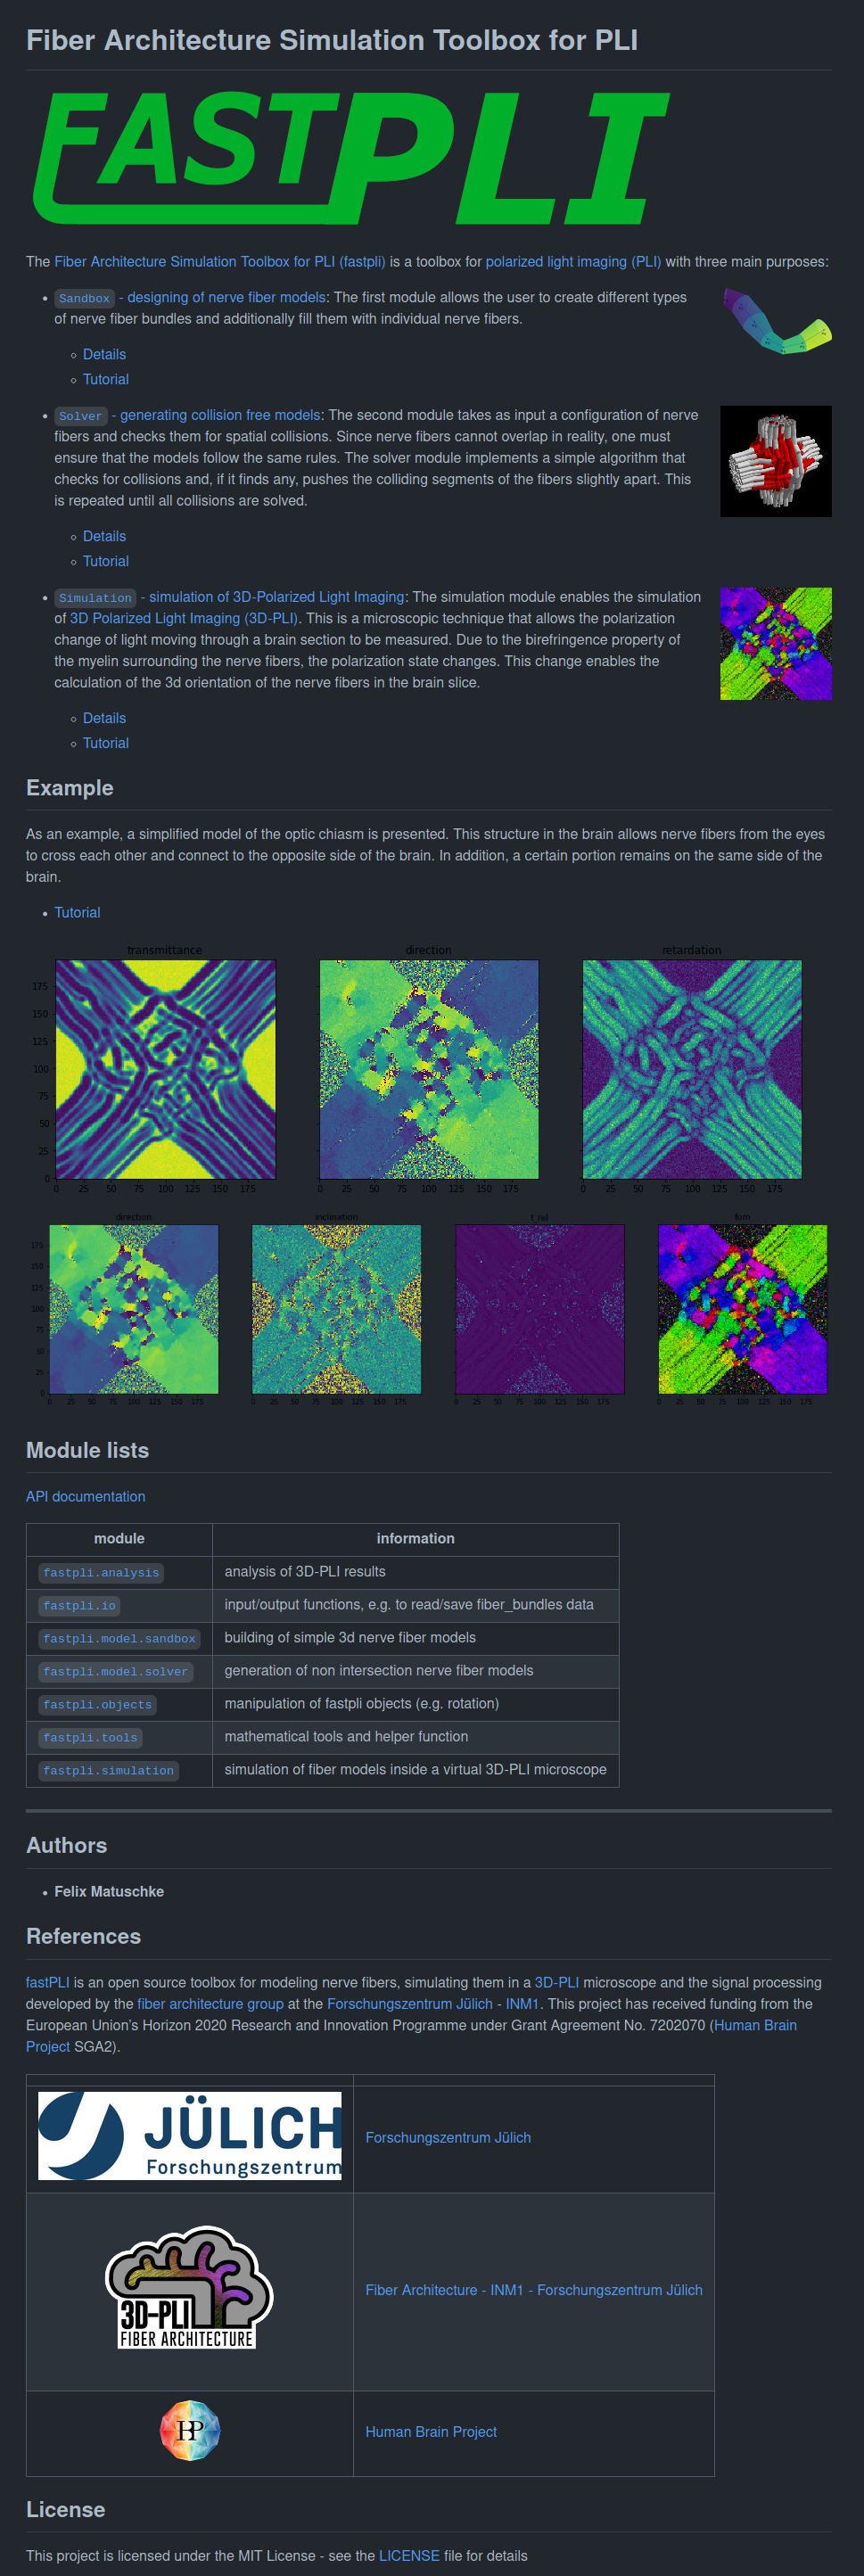
\includegraphics[valign=T,trim=0 1300 0 0, clip]{gfx/fastpli/fastpli_wiki.png} &
   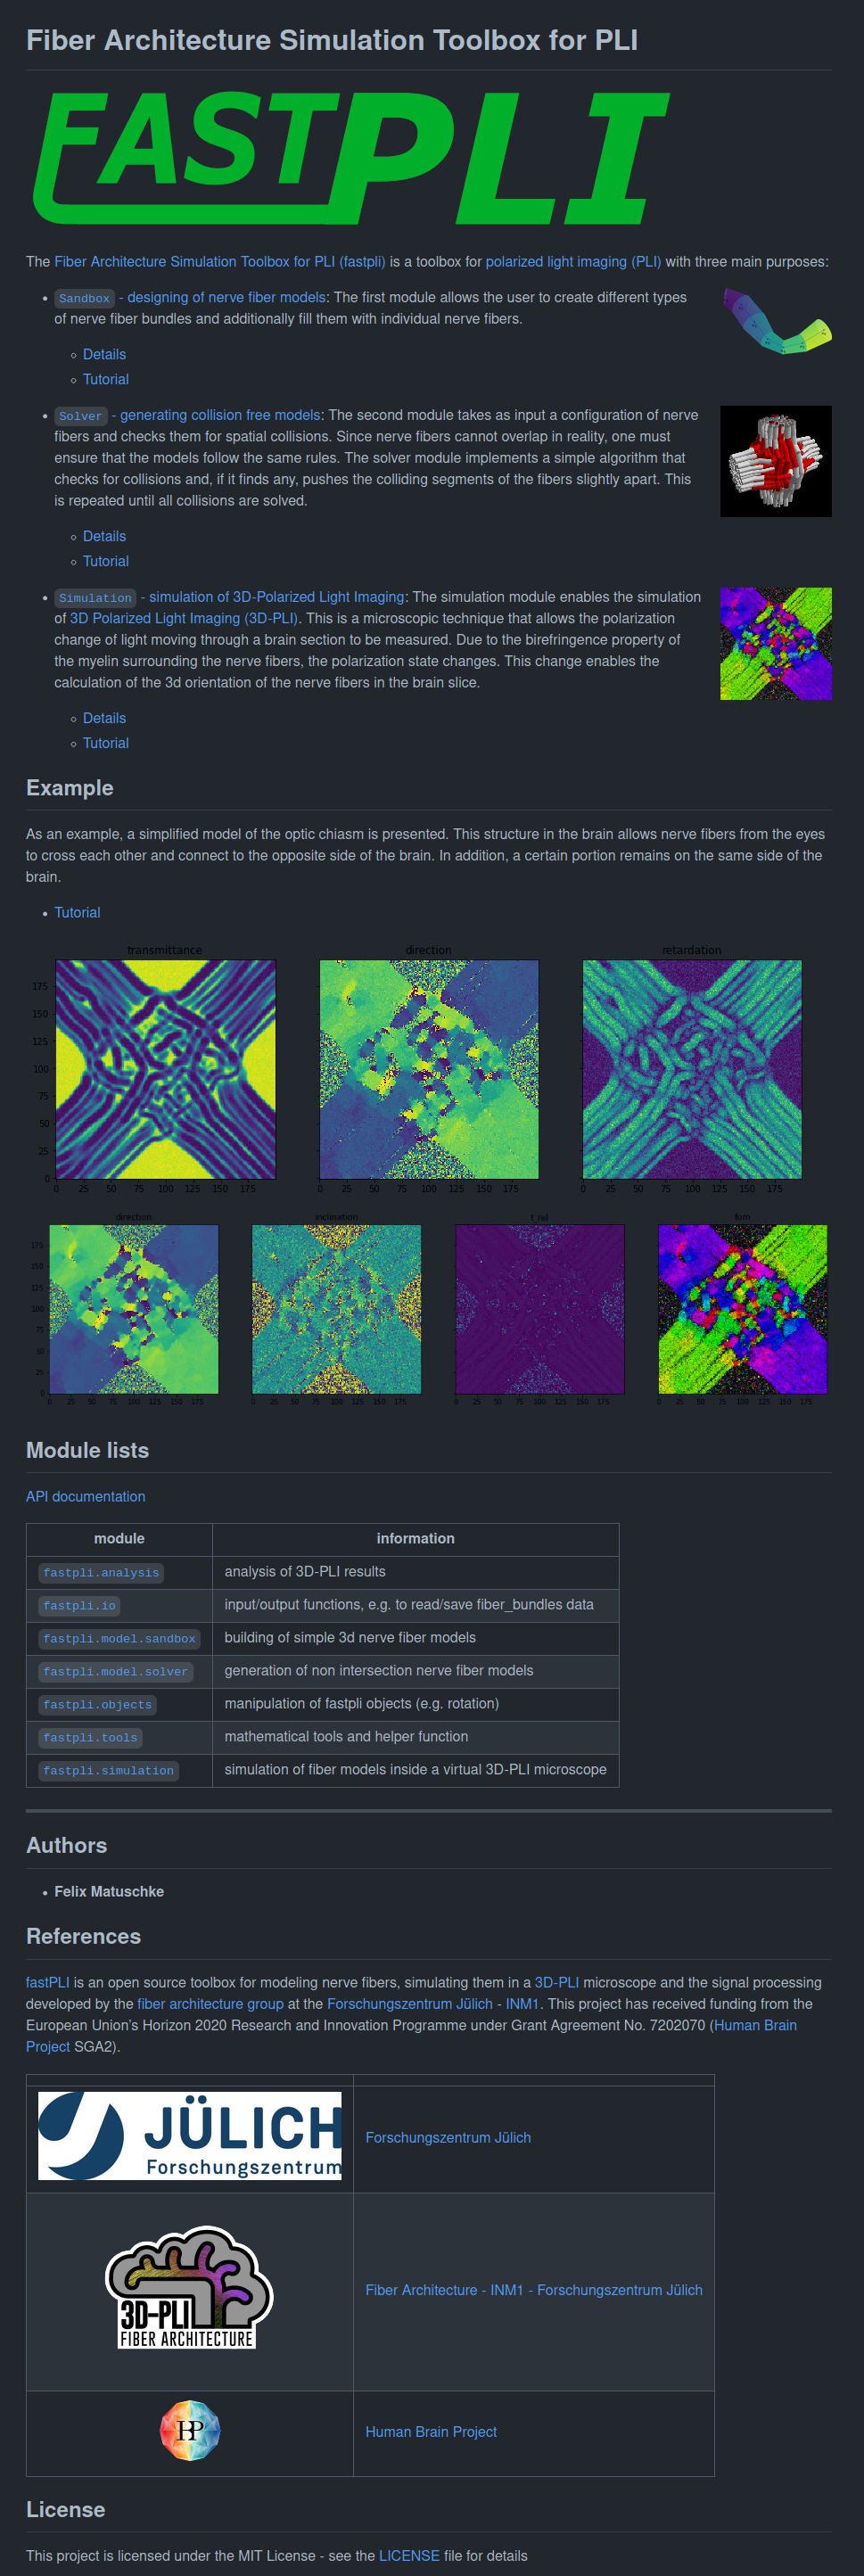
\includegraphics[valign=T,trim=0 0 0 1580, clip]{gfx/fastpli/fastpli_wiki.png} \\
   \end{tabular}
   }}
  \caption[]{Documentation wiki page of the \name{Github} repository \url{https://github.com/3d-pli/fastpli/wiki}.}
  \label{fig:fastpli_wiki}
\end{figure}
%
The wiki is an essential part of the review process for release in \ac{JOSS} \cite{Matuschke2021}, and it is structured as a guide that walks through the aspects of designing nerve fiber models, applying the collision solver algorithm, visualizing nerve fibers, an introduction in \ac{3D-PLI}, and finally applying the models in the simulation.
\par
%
Both executable \python{} scripts and Jupyter notebooks are provided examples for a friendly user familiarization with the tool. A nerve fiber crossing is presented as a general example using all presented methods. The example is based on the optic chiasm's anatomy, which is the nerve fiber pathway from the eyes to the occipital lobe.